\documentclass{beamer}
\usepackage{graphics}

\title{A Single-board computer using the AJIT lite processor \\ with an attached accelerator}
\author{Madhav Desai \\
Department of Electrical Engineering\\
IIT Bombay}

\begin{document}
\maketitle


\frame[containsverbatim]{\frametitle{The processor}
\begin{itemize}
\item AJIT 1x1x32 Lite:  AJIT single core, SPARC-V8 ISA.
\begin{itemize}
\item 8KB Icache (2-way set associative).
\item 8KB Dcache (2-way set associative).
\end{itemize}
\item Hardware debug support unit.
\item Integrated peripherals: interrupt controller, timer,
serial, scratch pad, performance counters, SPI master, I2C master.
\end{itemize}
}

\frame[containsverbatim]{\frametitle{Processor VHDL code hierarchy}
\begin{verbatim}
processor_1x1x32_lite
  mcore_1x1x32_lite
    core_1x32_no_fp_no_mmu
      munit_no_mmu
        dcache
        icache
        dummy_mmu
        mmu_mux
      cpu_no_fp
        teu_no_fp
        stream_corrector
\end{verbatim}
}
\frame[containsverbatim]{\frametitle{Processor VHDL code hierarchy}
\begin{verbatim}
        iunit
          iu_exec
          iu_registers
          iu_writeback_in_mux
        ifetch
        iretire
        loadstore
        idecode_idispatch
        dummy_fpunit
        ccu
        debug_interface 
  peripherals
\end{verbatim}
}

\frame[containsverbatim]{\frametitle{The top-level}

\begin{figure}
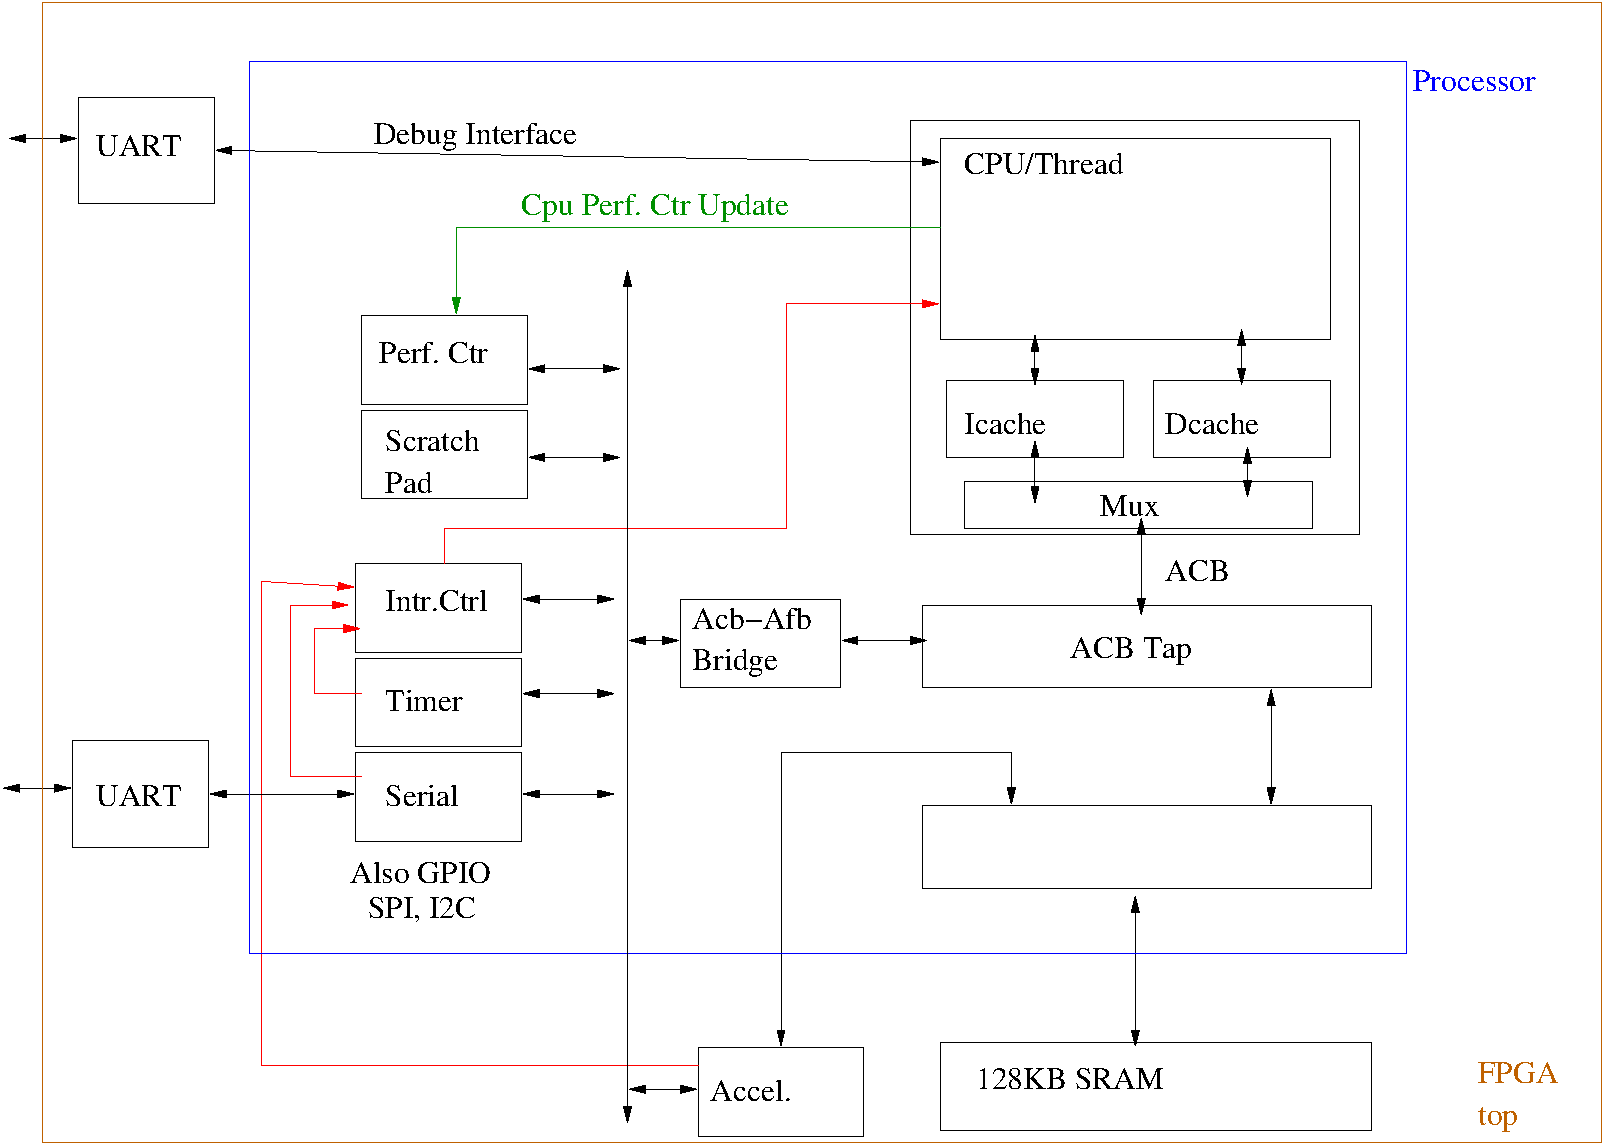
\includegraphics[width=10cm]{figs/fpga_top.pdf}
\end{figure}

}

\frame[containsverbatim]{\frametitle{The connections}

\begin{figure}
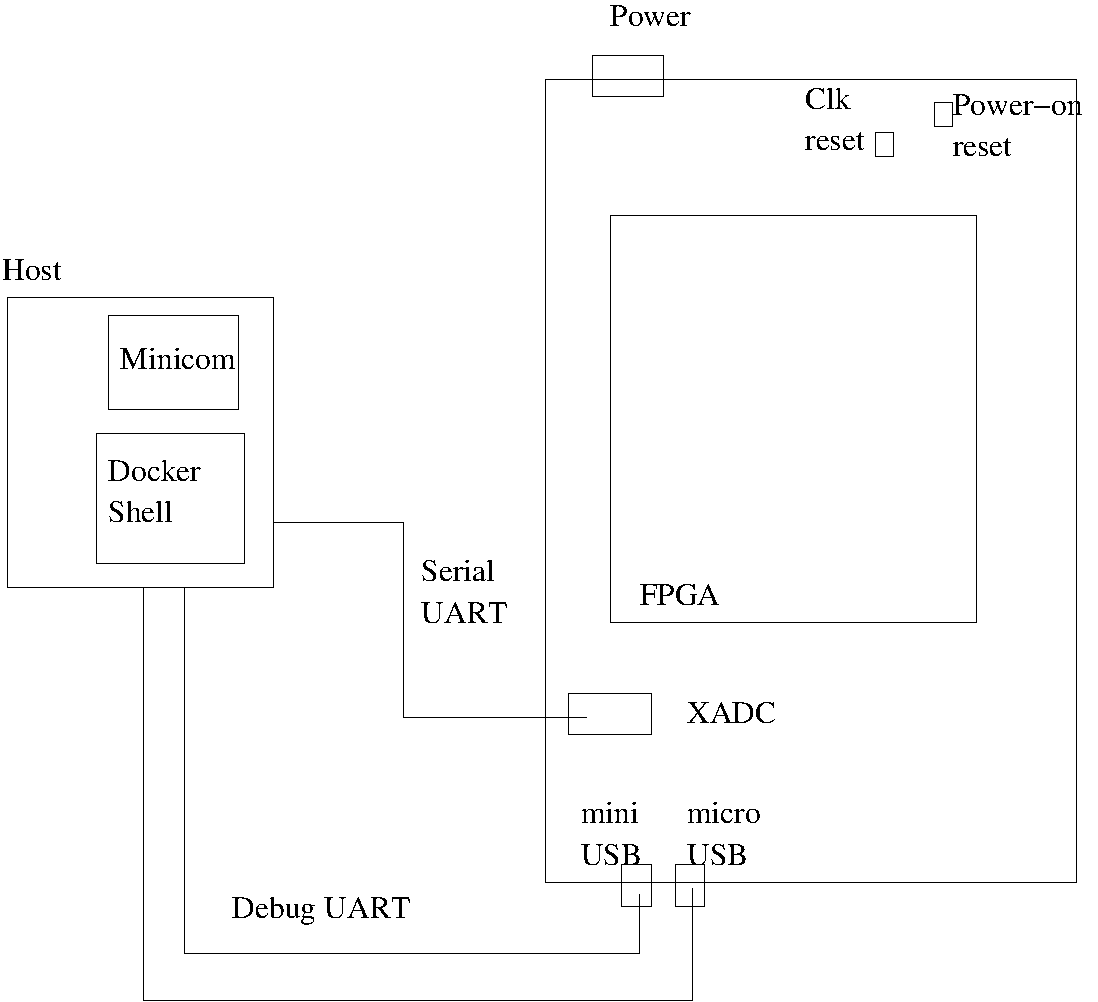
\includegraphics[width=8cm]{figs/connections.pdf}
 \caption{Connections}
\end{figure}

}


\frame[containsverbatim]{\frametitle{The connections: confirmation}

\begin{itemize}
\item Programming the FPGA (note the USB tty, suppose it is /dev/ttyUSBP).
\item Serial cable to FPGA (note the USB tty, suppose it is /dev/ttyUSBQ).
\item USB-UART (note the USB tty, suppose it is /dev/ttyUSBR).
\end{itemize}

}

\frame[containsverbatim]{\frametitle{The connections: summary}
\begin{itemize}
\item For FPGA programming, 1x USB (USB micro connector on FPGA board).
\item For debugging UART, 1x USB   (USB mini connector on FPGA board).
\item For serial UART, 1x USB-UART (preferably 1.8V/3.3V).
\item On host computer
\begin{itemize}
\item One docker shell, in which we will run ajit\_debug\_monitor\_mt
application.
\item One minicom terminal, set to 115200 baud.
\end{itemize}
\end{itemize}
}

\frame[containsverbatim]{\frametitle{First test program}
\begin{verbatim}
.section .text.ajitstart
_start:
mov 0x1, %g1
mov 0x2, %g2
add %g1, %g2, %g3
ta 0
\end{verbatim}

Compile this code to generate a memory map file.
}

\frame[containsverbatim]{\frametitle{Program the FPGA}
Start VIVADO and program using the bit-file
\begin{verbatim}
processor_1x1x32_lite.with_accelerator.kc705.bit
\end{verbatim}
}

\frame[containsverbatim]{\frametitle{Start the AJIT debug monitor}
\begin{verbatim}
calibrateUart /dev/ttyUSBQ
ajit_debug_monitor_mt /dev/ttyUSBQ
\end{verbatim}

This brings up a prompt.
\begin{verbatim}
[0:0]>
\end{verbatim}
}

\frame[containsverbatim]{\frametitle{Check if debug monitor is connected}

At the AJIT debug monitor prompt, type
\begin{verbatim}
[0:0]> r mode
\end{verbatim}
It should return $0$.

}

\frame[containsverbatim]{\frametitle{The AJIT debug monitor gives you access to all internal state}
\begin{itemize}
\item Read/write from any integer register.
\item Read/write from any state register (PSR, WIM, TBR, Y, ASR).
\item Read/write from any memory location, using any ASI.
\item The AJIT debug monitor also hooks up to a remote GDB client
and provides real-time debug capability.
\end{itemize}
}

\frame[containsverbatim]{\frametitle{Processor start sequence}
\begin{figure}
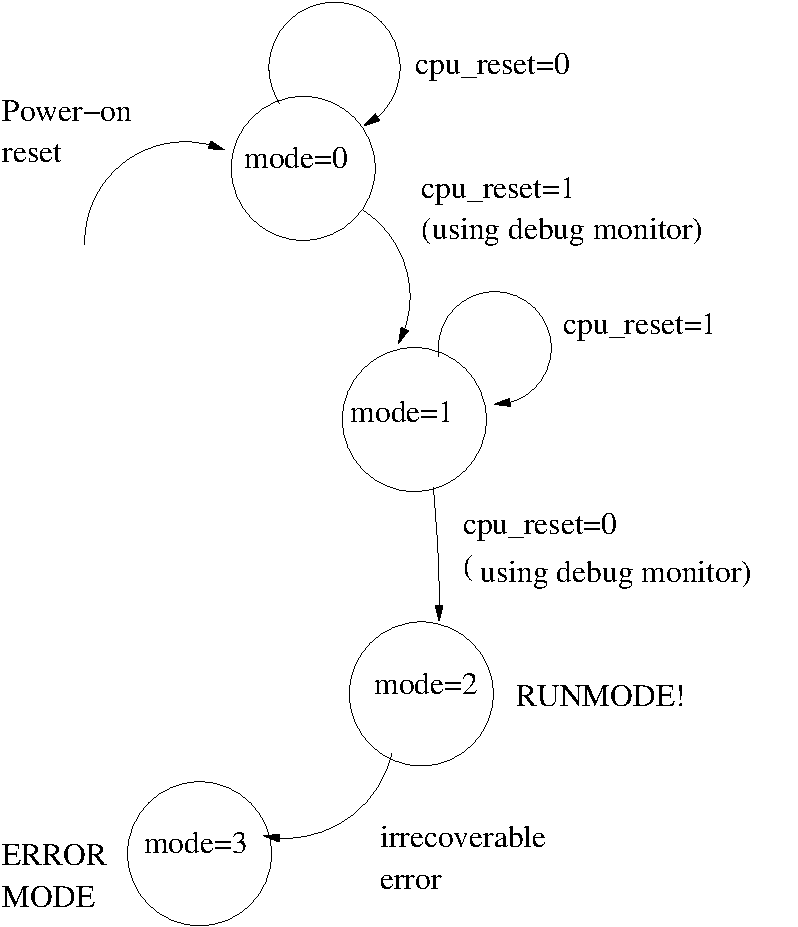
\includegraphics[width=6cm]{figs/startsequence.pdf}
 \caption{Start sequence}
\end{figure}
}


\frame[containsverbatim]{\frametitle{Run the debug monitor script}

\begin{verbatim}
[0:0]> s run.script
\end{verbatim}
The script makes CPU reset "1", downloads the memory map,
and then sets the CPU reset to "0", putting the CPU into
RUN mode (the LED's indicate this mode transition from 0 to
1 to 2 and then eventually 3.

The CPU mode LEDs then becomes 0x3, indicating that
the program has completed and the processor is halted in
error mode.  Read back register 3, ensure it holds value 0x3.
\begin{verbatim}
[0:0]> r iureg 3
\end{verbatim}
Should return 3.

}

\frame[containsverbatim]{\frametitle{Other post run observations}
\begin{itemize}
\item The processor is in mode 0x3 (error-mode).
\begin{itemize}
\item By default the processor is started with traps disabled.
Instruction at PC=0xc generates a trap with traps disabled.
The processor goes into error state and halts.
\item Registers g1, g2 hold values 0x1 and 0x2 respectively.
\begin{verbatim}
[0:0]> r iureg 1
[0:0]> r iureg 2
\end{verbatim}
\item The PSR will indicate that the processor is in window 7.  This
is the default window when the processor starts off, and it stays there.
\end{itemize}
\end{itemize}
}

\frame[containsverbatim]{\frametitle{Second test program: also a small assembly program}

\begin{itemize}
\item A GCD calculation program.
\item The example illustrates branches and delay slots.
\item Go through the whole sequence (given earlier).
\item Check that register 2 holds the final value, which is 0x1.
\item Processor halts in mode 0x3.
\item PSR window is 0x7.
\end{itemize}
}

\frame[containsverbatim]{\frametitle{Moving on: A bare-metal C program, the hello\_world benchmark} 

\begin{itemize}
\item We will print "Hello, world".
\item First we use an assembly file to set up the run-time that the C program requires
\begin{itemize}
\item Set up the stack.
\item Set up the WIM so that we use 8 windows.
\item Set up the PSR, enable traps.
\item Jump to the main program.
\item Trap on return.
\end{itemize}
\item We will have to supply trap handlers!
\item Compile and link.
\end{itemize}

}

\frame[containsverbatim]{\frametitle{Setting up the run-time} 
\begin{verbatim}
.section .text.ajitstart
.global _start;
_start: ! we reach here in window 7, post reset.
	set 0x20000, %fp  ! Stack
	sub %fp, 64, %sp  ! High Mem

	set 0x1, %l0      ! window 0 invalid
	wr %l0, 0x0, %wim

	set 0x10E7, %l0	  ! enable traps.
	wr %l0, %psr

	set trap_table_base, %l0
	wr %l0, 0x0, %tbr ! TBR

	call main
	nop
	ta 0   ! return here, goto error.
\end{verbatim}
}

\frame[containsverbatim]{\frametitle{Moving on: compiling and linking}
\begin{verbatim}
MAIN=hello_world
AAR=$AJIT_ACCESS_ROUTINES_MT
PT=$AJIT_MINIMAL_PRINTF_TIMER
INCLUDES="-I ../ -I ../include/ \
          "-I $AAR/include -I $PT/include "
SRCS=" -C ./ -C $AAR/src -C $PT/src -s \
          "  ./init.s -s ./trap_handlers.s"
DEFINES=" -D CLK_FREQUENCY=80000000 "

#Step 1: Generate the Linker Script
makeLinkerScript.py -t 0x0 -d 0x10000\
           -o customLinkerScript.lnk

#Step 2: Compile the application using uclibc
compileToSparcUclibc.py -o 3 -U -N ${MAIN} \
        $INCLUDES $SRCS $DEFINES \
        -L customLinkerScript.lnk
\end{verbatim}
}

\frame[containsverbatim]{\frametitle{Run it on hardware}
\begin{itemize}
\item But first, we need to start a terminal program (e.g. minicom)
for program I/O.
\begin{verbatim}
minicom -s
\end{verbatim}
\item Setup minicom for 115200 baud, connect to /dev/ttyUSBR.
\item In the Docker shell, run ajit\_debug\_monitor\_t as before.
\begin{itemize}
\item Power-on reset, calibrate UART as before.
\item Put CPU into reset.
\item Download memory map.
\item Move CPU out of reset.
\end{itemize}
\item You should see the print on the minicom.
\end{itemize}
}

\frame[containsverbatim]{\frametitle{Developing applications using CORTOS2}
\begin{itemize}
\item Describe the system configuration
\begin{itemize}
\item Hardware (ISA, number of cores, number of threads/core, MMU, FPU).
\item Memory regions (Flash, RAM, Non-cacheable RAM, IO).
\item Build options (stack size, debug, compiler flags, defines etc.).
\item Dynamic memory size.
\item Interrupt handlers.
\item Software trap handlers.
\end{itemize} 
\item CORTOS2 takes care of lower level details.
\item Program can use CORTOS2 routines for managing logging, printing, 
dynamic memmory management, locks, message queues.
\item Running the application on the FPGA follows same pattern as
above.
\end{itemize}
}

\frame[containsverbatim]{\frametitle{CORTOS2 examples}
\begin{itemize}
\item Hello world.
\item Display processor configuration, performance counters.
\item Illustrate use of GDB.
\item Serial interrupts.
\item Timer interrupts.
\item Software traps.
\item Accelerator.
\end{itemize}
}

\frame[containsverbatim]{\frametitle{Go through the examples one by one}

For each example we review:
\begin{itemize}
\item The configuration.
\item The program.
\item The build process.
\item Using the AJIT debug monitor to run the program.
\item For one of the examples, illustrate the use of
the debugger.
\end{itemize}

}

\end{document}
